\documentclass[12pt,letter]{article}
\usepackage{../downey_format}

\begin{document}

	% set the section number, along with figure and equation numbers
	\setcounter{section}{3}	
	\setcounter{figure}{0}   
	\renewcommand\thefigure{\thesection.\arabic{figure}}
	\setcounter{equation}{0}   
	\renewcommand\theequation{\thesection.\arabic{equation}}

\section{Regression-Based Classification}

Certain algorithms that were first developed for regression can be adapted for classification, and some classifiers can be modified to predict continuous values. Converting a linear regressor into a classifier by adding a logistic link, for instance, retains the original coefficient vector, which makes it easy to see how each input feature influences the decision. As these dual-purpose models expose many of the hyper-parameters found in their regression versions, they often provide more opportunities for fine-tuning and clearer interpretability than algorithms designed purely for classification.

\subsection{Logistic Regression}


Logistic Regression, sometimes called logit regression, models the probability that a sample belongs to a specific class, such as the chance that an email is spam. When this probability exceeds 50\%, the model predicts the positive class (label~``1''); otherwise, it predicts the negative class (label~``0''). It therefore acts as a binary classifier.


The predicted probability is
\begin{equation}
    \hat{p} = h_\theta(X) = \sigma(\theta^\text{T} \cdot X).
\end{equation}
Here $\hat{p}$ is the estimated probability, and $\sigma(\cdot)$ is the sigmoid function, an $S$-shaped curve that maps any real number to the interval $(0,1)$. The logistic function is defined in Equation~\ref{eq:logistic_function} and illustrated in Figure~\ref{fig:sigmoid_function}. As before, $h_\theta(X)$ denotes the hypothesis that the input matrix $X$, augmented with a bias term, belongs to the positive class under the parameters~$\theta$.


\begin{equation}
    \sigma(x) = \frac{1}{1 + e^{-x} }.
    \label{eq:logistic_function}
\end{equation}


		\begin{figure}[H]
			\centering
			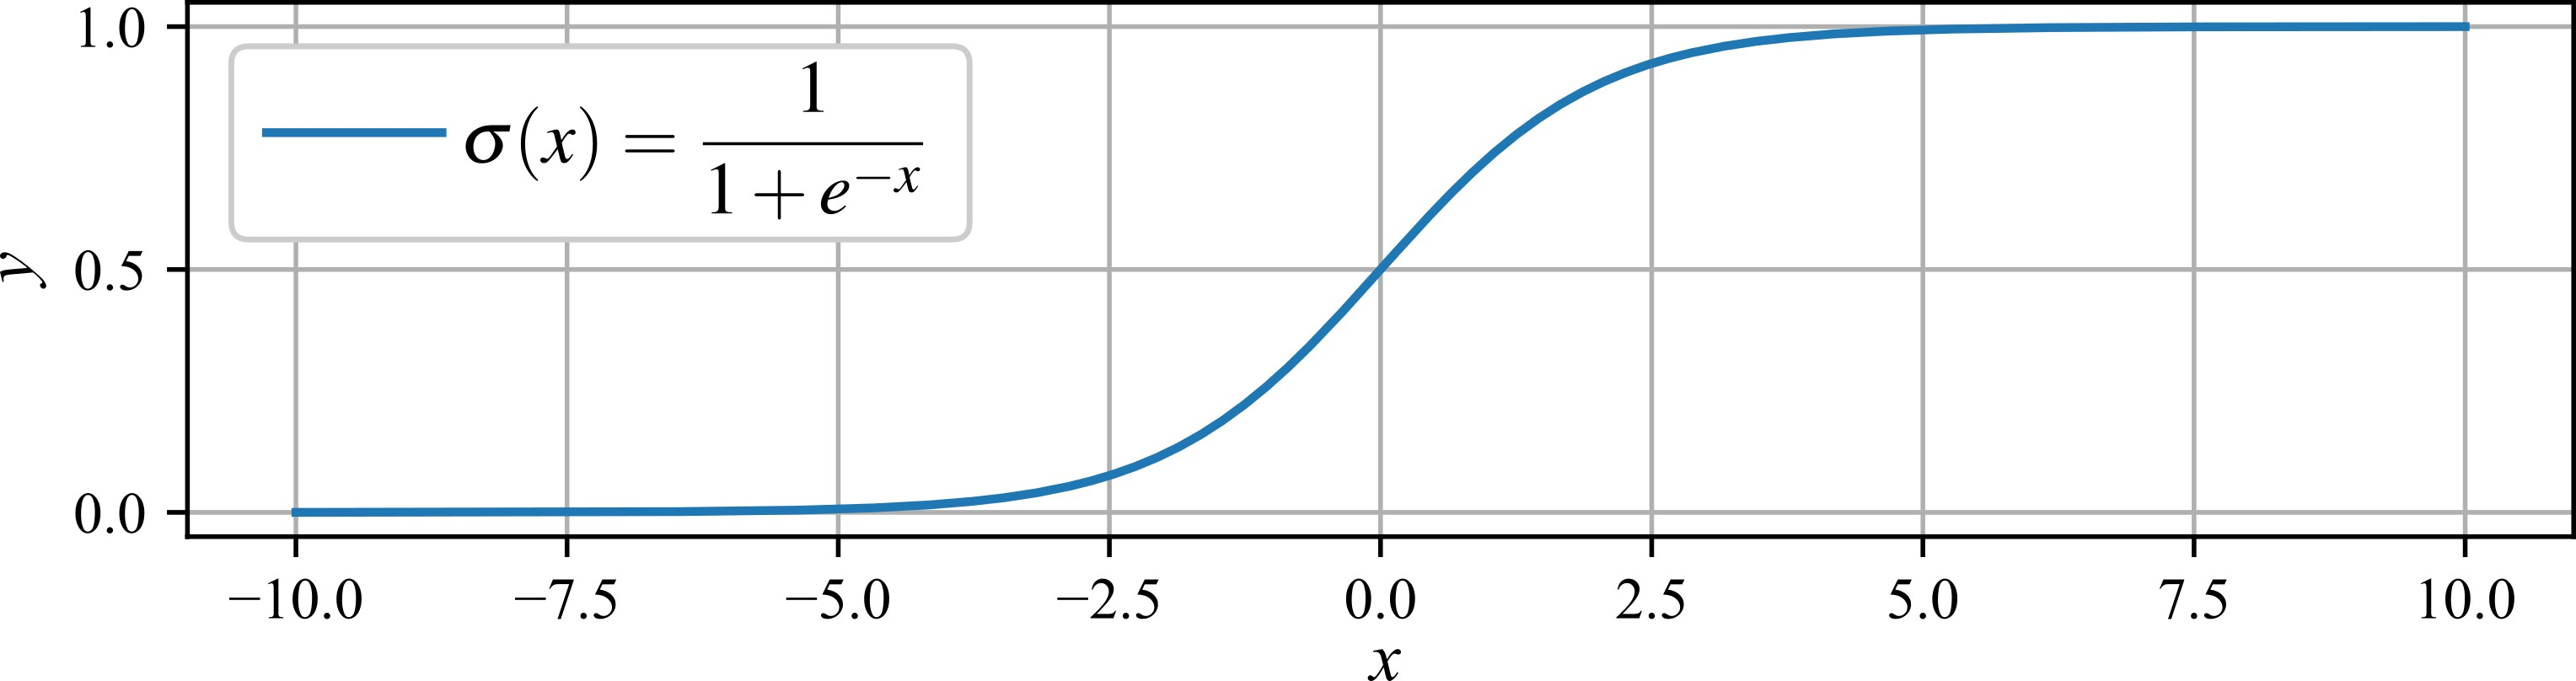
\includegraphics[width=6.1in]{../figures/sigmoid_function}
			\caption{Sigmoid function that maps any real-valued input $x$ to a value between 0 and 1. }
			\label{fig:sigmoid_function}
		\end{figure}

Once the probability $\hat{p} = h_\theta(X)$ that an instance $X$ belongs to the positive class has been estimated using Logistic Regression, the prediction ($\hat{y}$) can be made. $\hat{y}$ is calculated as
\begin{equation}
  \hat{y} = 
  \begin{cases}
  0 & \text{if } \hat{p} < 0.5, \\
  1 & \text{if } \hat{p} \ge 0.5.
  \end{cases}
\label{eq:model_prediction}
\end{equation}
Note that $\sigma(x) < 0.5$ when $x < 0$, and $\sigma(x) \ge 0.5$ when $x \ge 0$. Therefore, the Logistic Regression model predicts 0 if $\theta^\text{T} \cdot X$ is negative, and 0 if it is positive.

Now that we understand how logistic regression assigns probabilities and produces predictions, let's walk through a concise example that shows its training procedure and the associated cost function.
Training seeks parameter values $\theta$ that give high predicted probabilities to positive examples ($y = 1$) and low probabilities to negative ones ($y = 0$). This aim is captured by the cost defined in equation~\ref{eq:cost_function}, which evaluates a single training sample $x$. To achieve this, we require a cost function, such as 
\begin{equation}
  C(\theta) = 
  \begin{cases}
  - \log (\hat{p}) & \text{if } y=1, \\
  - \log (1-\hat{p}) & \text{if } y=0.
  \end{cases}
\label{eq:cost_function}
\end{equation}
The considered cost function is plotted in figure~\ref{fig:Logistic_Regression_cost_function}.

\begin{figure}[H]
	\centering
	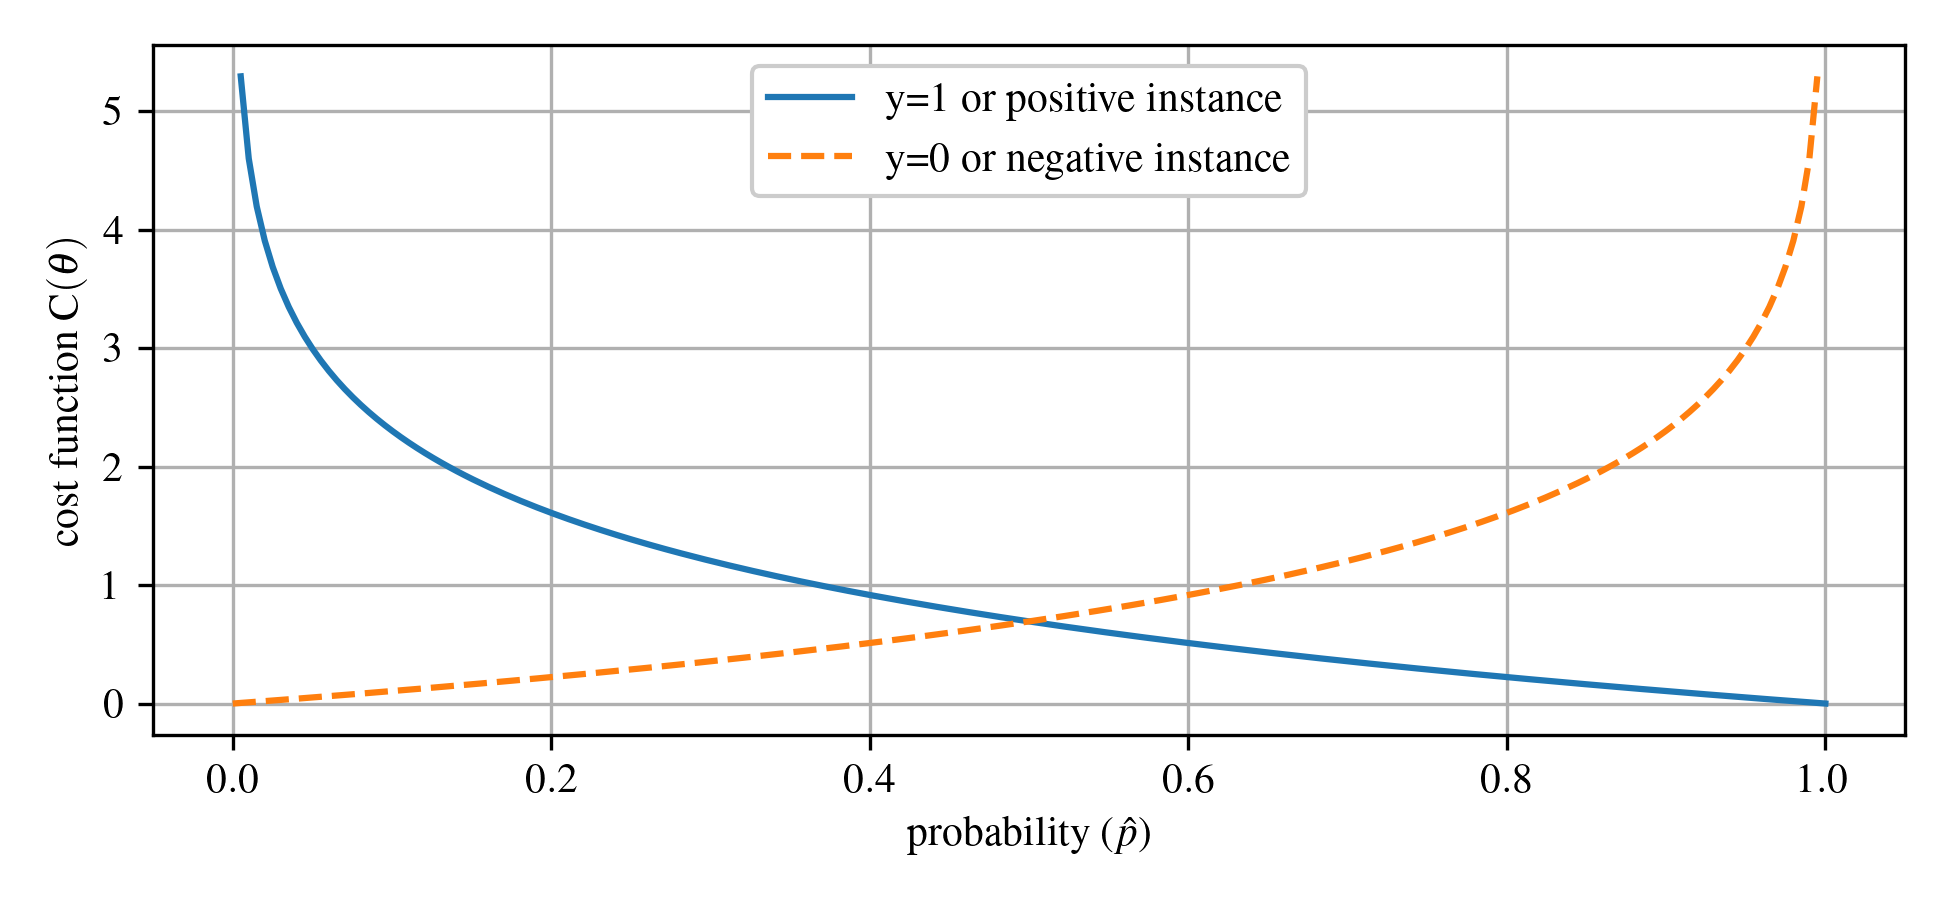
\includegraphics[width=5.5in]{../figures/Logistic_Regression_cost_function.png}
	\caption{Cost function behavior for classification that heavily penalizes incorrect predictions.}
	\label{fig:Logistic_Regression_cost_function}
\end{figure}

The cost function in equation~\ref{eq:cost_function} behaves intuitively: $-\log(\hat{p})$ increases sharply as $\hat{p} \to 0$, so the loss is large when the model assigns a probability near0 to a positive example. It likewise produces a high loss when the model predicts a probability close to1 for a negative example. Conversely, because $-\log(\hat{p})\to0$ as $\hat{p} \to 1$, the loss becomes negligible when the predicted probability is near1 for a positive instance or near0 for a negative one, aligning with our expectations.



The overall cost, denoted $J(\theta)$, is the mean loss across all $m$ training examples. This metric is commonly called the log-loss and written as 
\begin{equation}
J(\theta) ;=; -\frac{1}{m}\sum_{i=1}^{m}\Big[y^{(i)} \log \bigl(\hat{p}^{(i)}\bigr) ;+; \bigl(1 - y^{(i)}\bigr) \log \bigl(1-\hat{p}^{(i)}\bigr)\Big].
\label{eq:log_loss}
\end{equation}

Because there is no closed-form solution for the parameters $\theta$ (embedded within $\hat{p}$), the minimum must be found with an iterative optimizer. The cost surface is convex, so gradient descent or another suitable algorithm will reach the global minimum provided the learning rate is reasonable and enough iterations are allowed. The gradient of the cost with respect to the $j^\text{th}$ parameter $\theta_j$ is given as
\begin{equation}
\frac{\partial J}{\partial \theta_j} ;=; \frac{1}{m} \sum_{i=1}^{m} \Bigl[\sigma \bigl(\theta^\text{T}X^{(i)}\bigr) - y^{(i)}\Bigr],x^{(i)}_{j}.
\label{eq:Logistic_cost_function_partial_derivatives}
\end{equation}


This equation resembles the partial derivative used in gradient descent. For every training example, it finds the prediction error, multiplies it by the $j^\text{th}$ feature value, and then averages these products over all $m$ samples. With the resulting gradient vector of partial derivatives, you can update the parameters using the Batch Gradient Descent algorithm, completing the training of a Logistic Regression model. Stochastic Gradient Descent performs the update after each single example, while Mini-batch Gradient Descent updates the parameters after processing each mini-batch.



\begin{data}
\textbf{Iris Flower Dataset}

\noindent The Iris dataset, collected by botanist Edgar Anderson in 1935, lists sepal length, sepal width, petal length, and petal width for 150 flowers drawn equally from three species: Iris-Setosa, Iris-Versicolor, and Iris-Virginic  (refer to Figure~\ref{fig:iris_species})a. Statistician Ronald Fisher analysed these measurements in a 1936 study on linear discriminant analysis, and the data have since become a standard benchmark in statistics and machine learning because they are small, clean, and perfectly balanced, making them ideal for testing classification algorithms and visualisation techniques.




\begin{figure}[H]
    \centering
    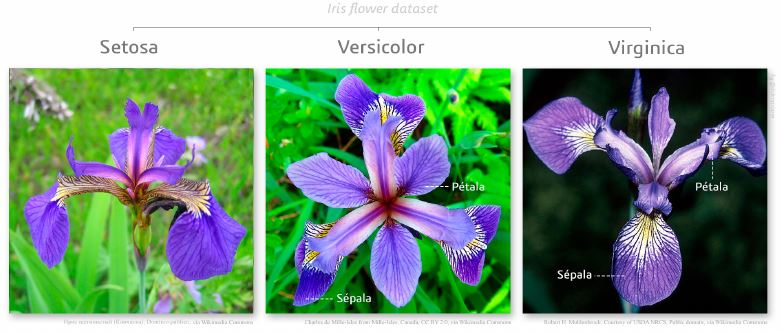
\includegraphics[width=5.5in]{../figures/iris_species.jpg}
    \caption{Flowers representing three species of iris plants \protect\footnotemark[1]}
    \label{fig:iris_species}
\end{figure}

		\begin{figure}[H]
			\centering
			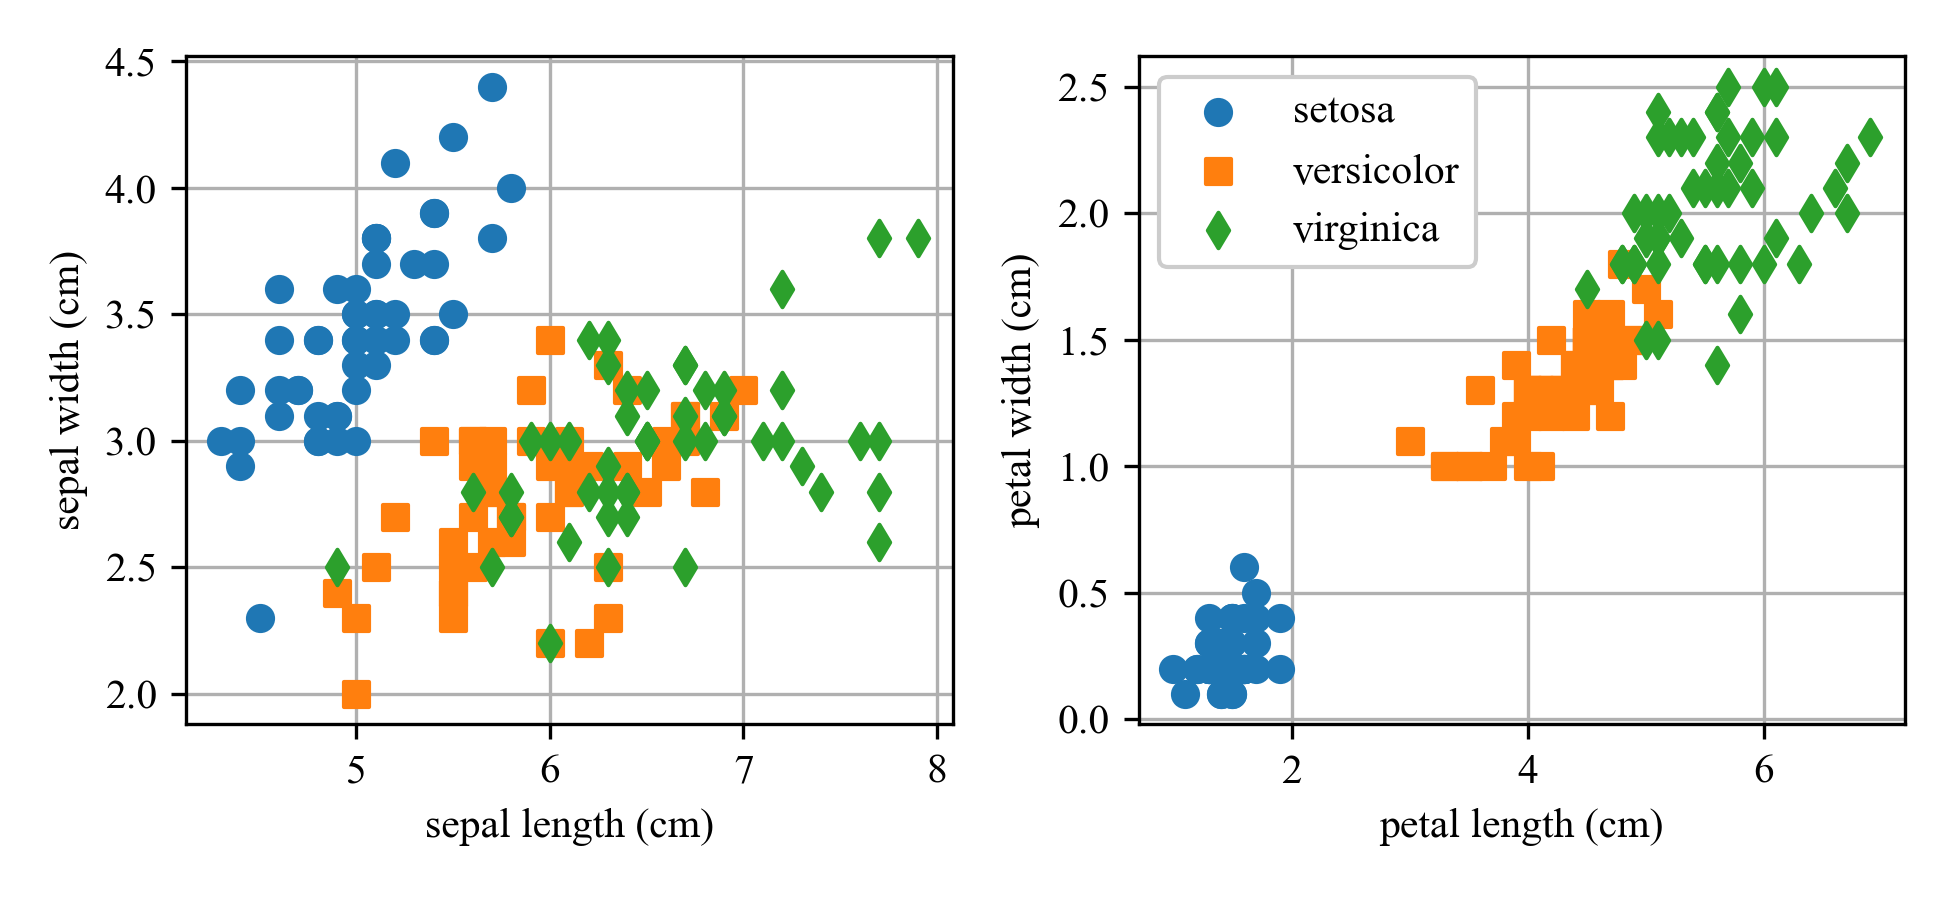
\includegraphics[width=5.5in]{../figures/Iris_dataset_scatterplot.png}
			\caption{Iris dataset scatterplot showing sepal length vs. sepal width (left) and petal length vs. petal width (right).  }
			\label{Iris_dataset_scatterplot}
		\end{figure}

\footnotetext[1]{Diego Mariano, CC BY-SA 4.0 $<$https://creativecommons.org/licenses/by-sa/4.0$>$, via Wikimedia Commons}
\end{data}



\begin{example}
\textbf{Iris Dataset Exploration}

\noindent This example introduces the Iris dataset (Figure~\ref{fig:iris_species}), originally compiled by Ronald Fisher. It demonstrates how to load the dataset, access feature and label information, and visualize the relationships between sepal and petal measurements across the three iris species.
\end{example}

\subsubsection{1-D Decision Boundaries}

The petal width of Iris-virginica flowers usually lies between 1.4~cm and 2.5~cm, whereas the other two species range from 0.1~cm to 1.8~cm. Because these intervals overlap, the classifier's certainty changes across the scale. Above roughly 2~cm, the model is confident that any given sample is Iris-virginica. Moreover, below 1~cm it is equally sure the flower is not Iris-virginica (This means the model redicts high probability for the class ``Not Iris-Virginica''). In between the limits of the classes, the model is unsure. When you call \texttt{predict()} instead of \texttt{predict\_proba()}, it outputs the most likely class, creating a decision boundary around 1.6~cm where both class probabilities reach 50~percent. Thus, flowers with petal widths greater than 1.6~cm lead to a prediction of Iris-virginica, while flowers with smaller petal widths yield the opposite prediction even if confidence is low.


\begin{figure}[H]
	\centering
	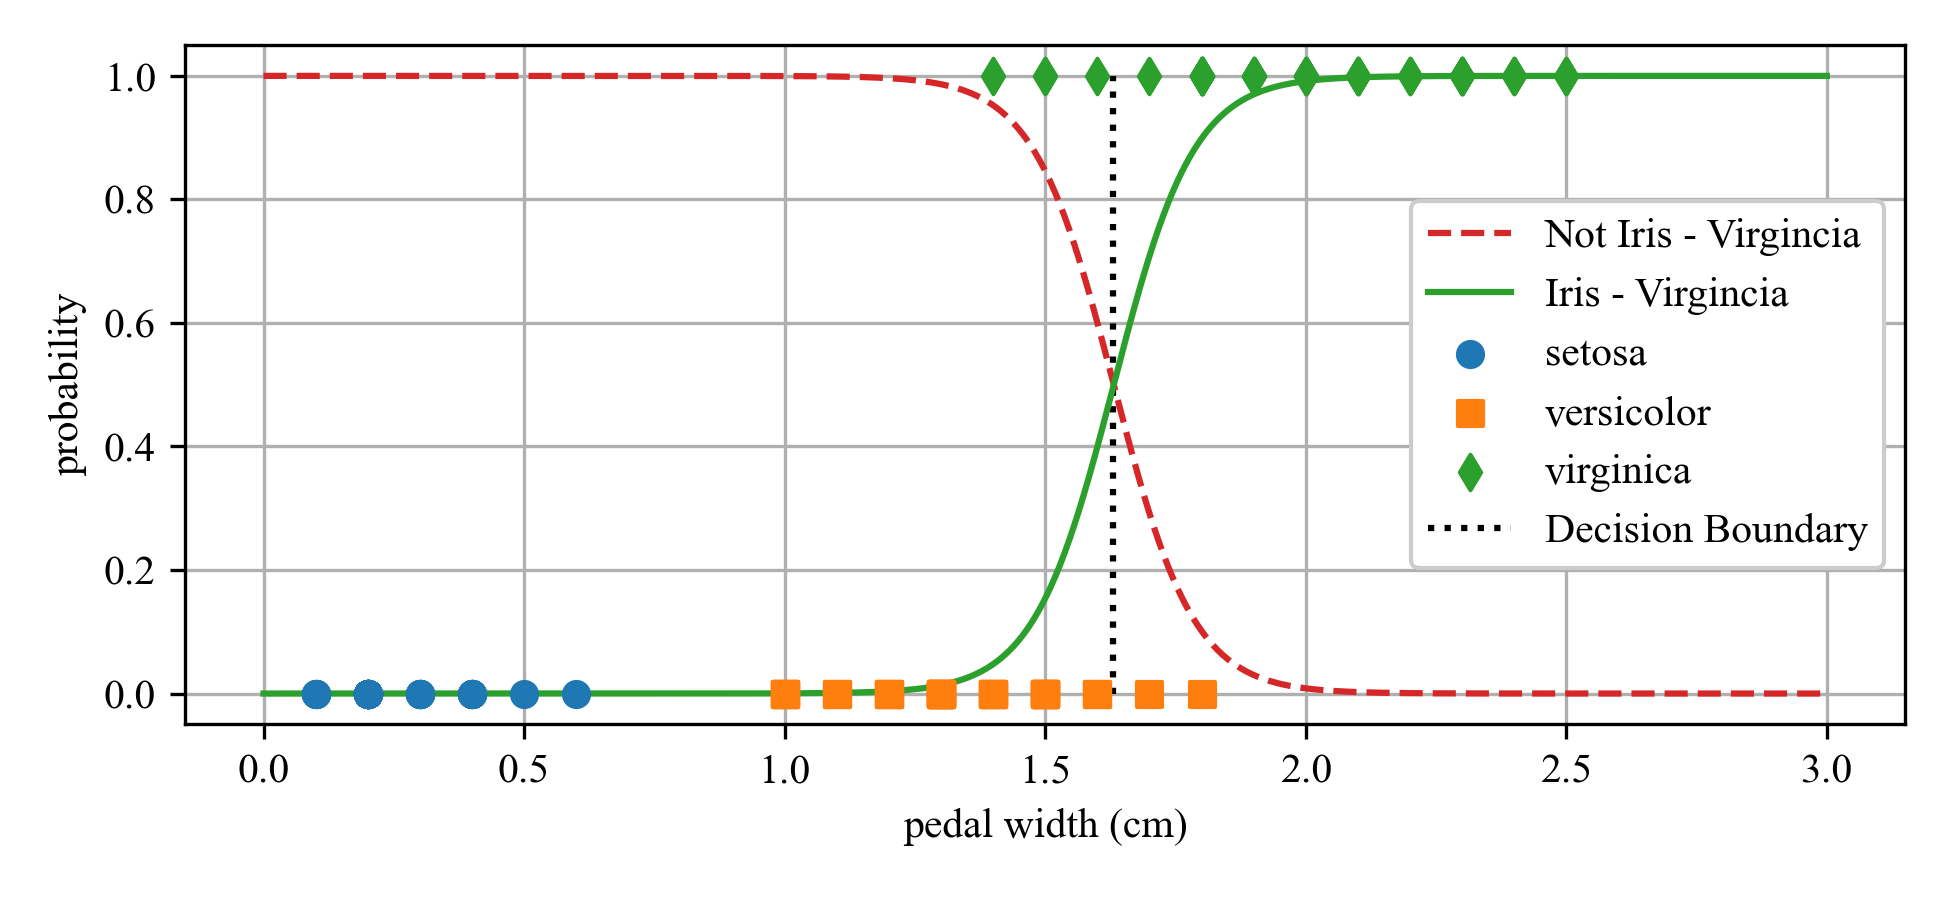
\includegraphics[width=6.2in]{../figures/Iris_dataset_decision_boundary_1D.png}
	\vspace{-3ex}
	\caption{Decision boundary for the flowers of three Iris plant species with C set to $C=10^{10}$ .}
	\label{fig:Iris_dataset_decision_boundary_1D}
\end{figure}

\vspace{-2ex}
\begin{example}
\textbf{1D Logistic Regression}

\noindent This example builds a logistic regression model to classify Iris-Virginica based on a single feature: petal width. It visualizes class probabilities and shows the decision boundary at the 50\% threshold.
\end{example}

	\vspace{-2ex}
\subsubsection{2-D Decision Boundaries}


Figure~\ref{fig:Iris_dataset_decision_boundary_2D} plots petal width against petal length for the Iris samples. After training, the logistic regression model assigns each point the probability that the flower is \textit{Irisvirginica}. The dashed line marks where this probability equals50 \%, forming the decision boundary, which is linear. The parallel contour lines show equal-probability levels from 10\% to 90\%. Points be beyond the top-right line have a greater than 90\% probability  of being classified as Iris-Virginica by the model.



		\begin{figure}[H]
			\centering
			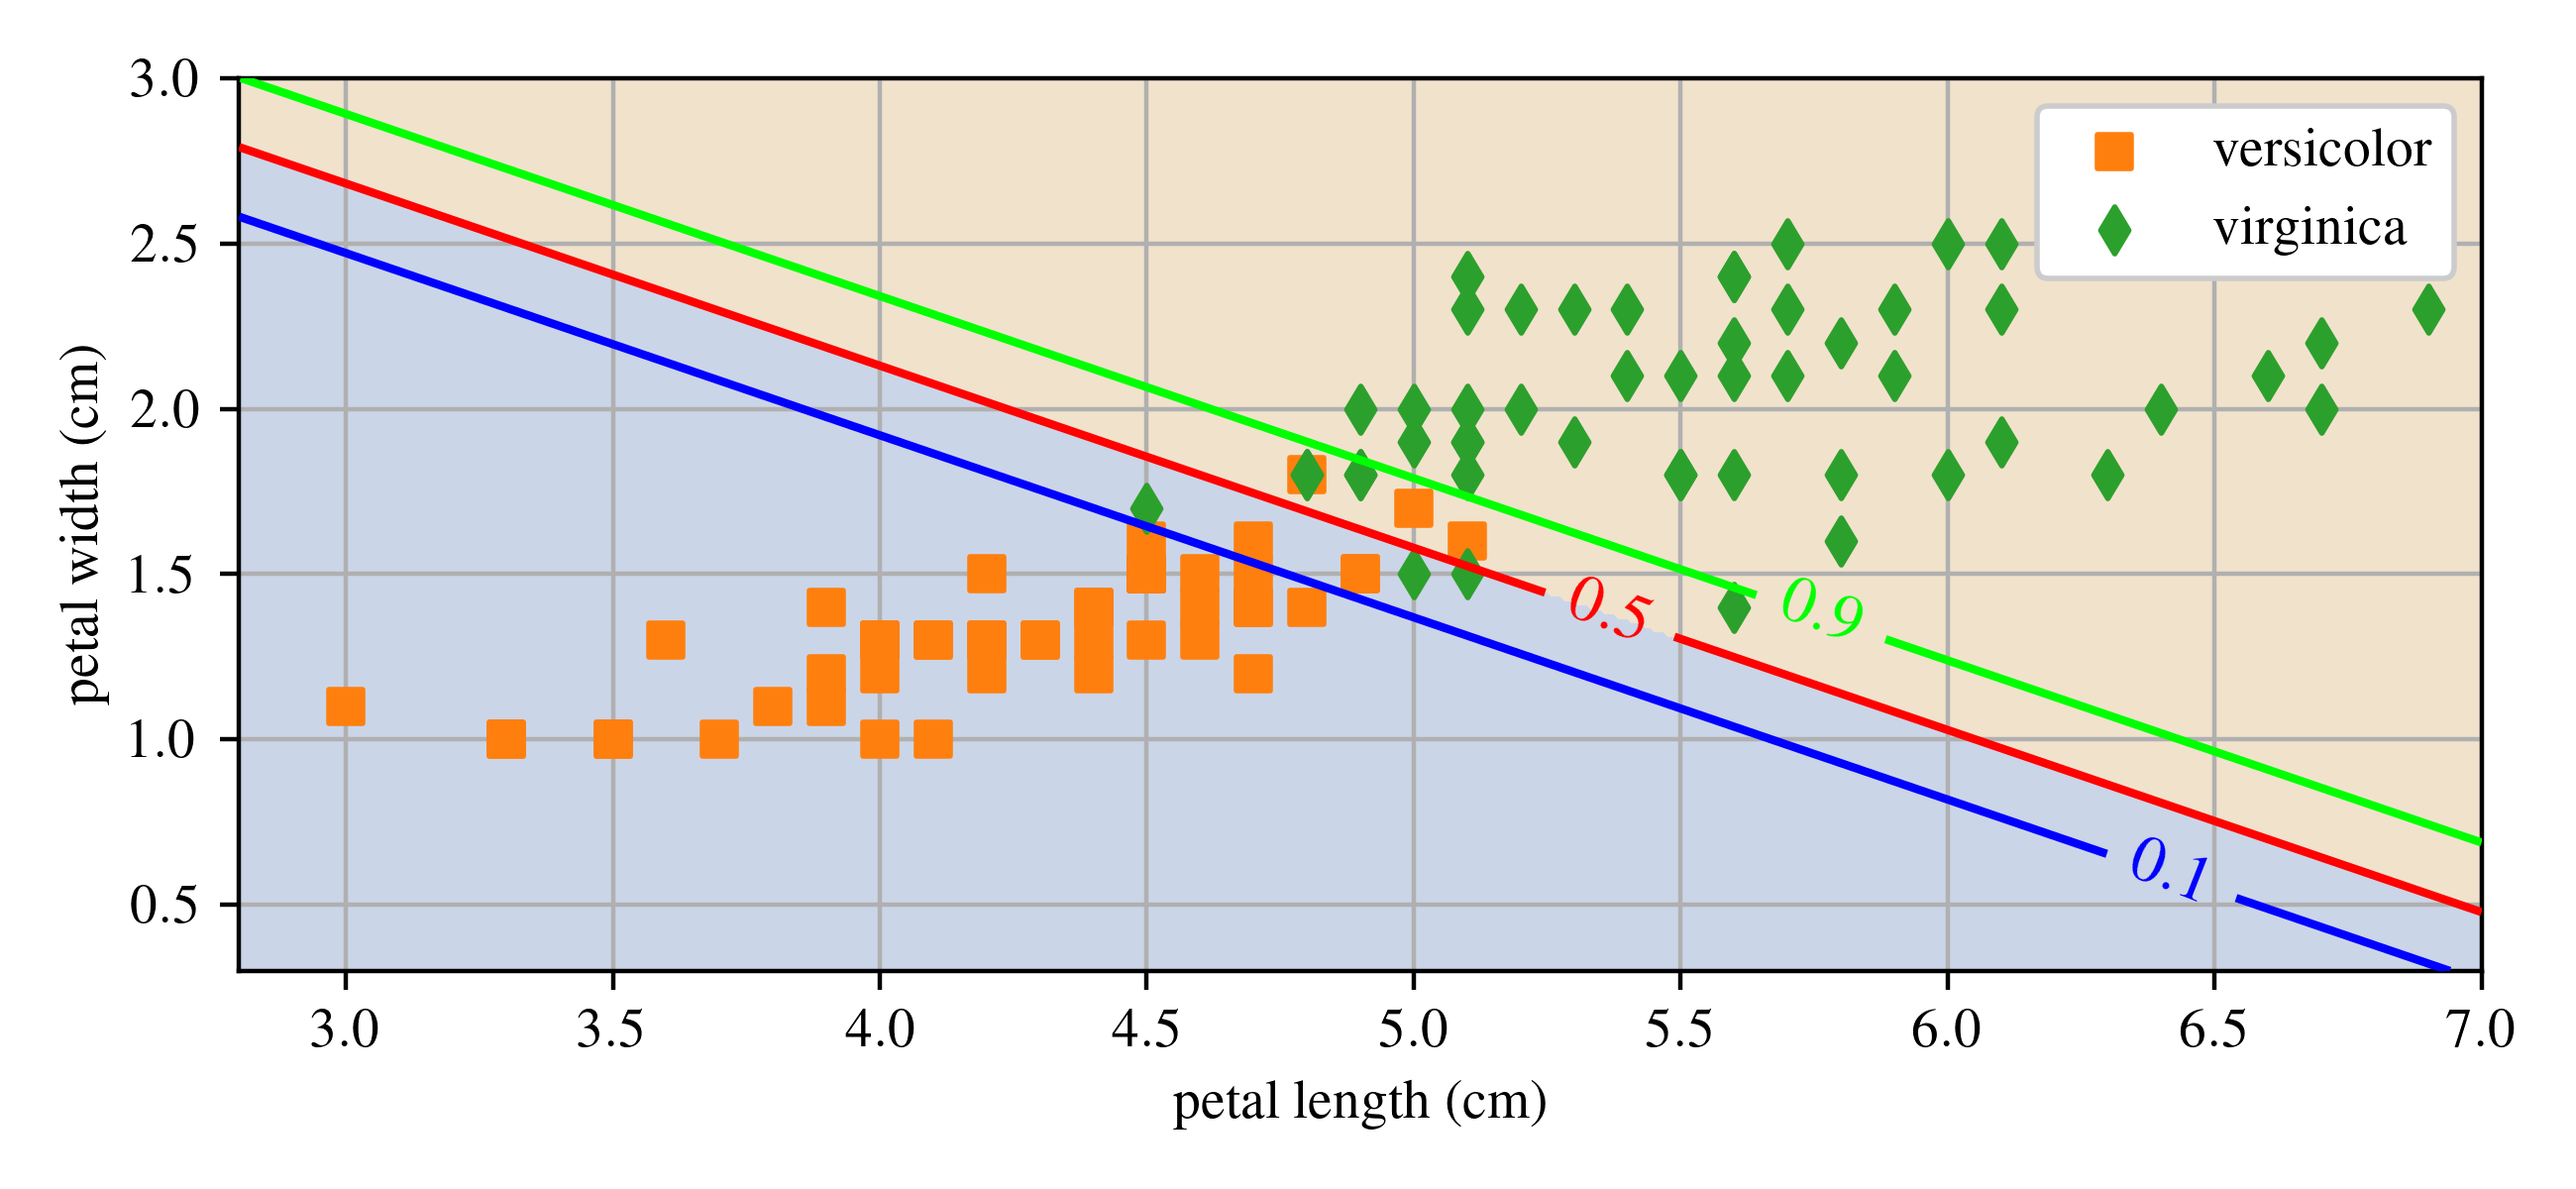
\includegraphics[width=6.2in]{../figures/Iris_dataset_decision_boundary_2D.png}
			\vspace{-3ex}
			\caption{A 2D decision boundary for the Iris dataset.}
			\label{fig:Iris_dataset_decision_boundary_2D}
		\end{figure}

\pagebreak

\begin{example}
\textbf{2D Decision Boundary}

\noindent This example uses logistic regression to classify the Iris-Virginica species based on petal length and width. A 2D decision boundary is visualized in the petal feature space, with prediction regions and probability contours illustrating classifier confidence.
\end{example}



\subsection{Softmax Regression}

Logistic Regression can be generalised to handle many classes in a single model, so there is no need to train and merge several binary classifiers. This multiclass version is called Softmax Regression, or Multinomial Logistic Regression. Softmax Regression provides a straightforward way to perform regression-based classification when more than two classes are present. For an input vector $\mathbf{x}$, the model first computes a score $s_k(\mathbf{x})$ for every class $k$, then turns these scores into class probabilities with the softmax (normalised exponential) function. The score is obtained exactly as in linear regression:
\begin{equation}
s_k(\textbf{x}) = \textbf{x}^\text{T}\pmb{\theta}^{(k)}.
\end{equation}
Here each class has its own parameter vector $\boldsymbol{\theta}^{(k)}$, and the collection of these vectors is usually stored as the rows of a parameter matrix $\Theta$.

After the model has calculated a score for each class given an input $\mathbf{x}$, it converts these scores to probabilities with the softmax function. For class $k$ the predicted probability is
\begin{equation}
\hat{p}_k = \sigma\big(s(\textbf{x}) \big)_k = \frac{\exp \big(s_k(\textbf{x})\big)}{\sum_{j=1}^{K} \exp \big(s_j(\textbf{x}) \big)}.
\label{eq:softmax}
\end{equation}
In this expression, $\mathbf{s}(\mathbf{x})$ is the vector of class scores for the input, $\sigma\bigl(\mathbf{s}(\mathbf{x})\bigr)_k$ is the probability that $\mathbf{x}$ belongs to class $k$, and $K$ is the total number of classes. In short, equation~\ref{eq:softmax} exponentiates each score and then normalises the results by dividing by the sum of all exponentials so the probabilities sum to one.


Like logistic regression, a Softmax~Regression model assigns an input to the class whose predicted probability is largest, which coincides with the class that has the highest score:
\begin{equation}
\hat{y} = \mathop{\text{argmax}}_{k} \sigma \big(\textbf{s}(\textbf{x})\big)_k = \mathop{\text{argmax}}_{k} s_k(\textbf{x}) = \mathop{\text{argmax}}_{k} \big( (\theta^{(k)})^\text{T} \cdot \textbf{x} \big).
\end{equation}


\begin{mdframed}[middlelinewidth=0.5mm]
\begin{center}
\bl{NOTE}
\end{center}
The argmax operator returns the argument that maximises a function. In this setting, it yields the index $k$ for which the estimated probability $\sigma \bigl(s(\mathbf{x})\bigr)_k$ attains its largest value.
\end{mdframed}



With probability estimation and prediction established, we next consider training. The task is to learn parameters that place a large probability on the correct class and correspondingly small probabilities on all others. This objective is met by minimising the cost in equation~\ref{eq:cross_entropy_cost_function}, known as the cross entropy, which heavily penalises the model when it assigns a low probability to the true label. Cross entropy is widely used to measure how well predicted class probabilities agree with the actual classes. The cost function is
\begin{equation}
J(\Theta) = -\frac{1}{m} \sum_{i=1}^{m} \sum_{k=1}^{K} y_k^{(i)} \log (\hat{p}_k^{(i)}).
\label{eq:cross_entropy_cost_function}
\end{equation}

\begin{mdframed}[middlelinewidth=0.5mm]
\begin{center}
\bl{NOTE}
\end{center}
In this expression, $y_k^{(i)} = 1$ when the $i^\text{th}$ sample's true label is class $k$, and $y_k^{(i)} = 0$ otherwise.
\end{mdframed}
When considering only two classes ($K = 2$), it's important to highlight that this cost function aligns with the Logistic Regression's cost function, commonly referred to as log loss (refer to Equation~\ref{eq:log_loss}).

The gradient of the cross-entropy cost with respect to $\boldsymbol{\theta}^{(k)}$ is
\begin{equation}
\nabla_{\theta^{(k)}}J(\Theta) = \frac{1}{m} \sum_{i=1}^{m} (\hat{p}_k^{(i)}-y_k^{(i)} X^{(i)}).
\end{equation}
By computing this vector for each class, you obtain the full gradient, which can then be fed to Gradient~Descent or another optimizer to find the parameter matrix $\Theta$ that minimises the cost.




Applying Softmax Regression to the three-class iris problem in Scikit-Learn is straightforward. The \texttt{LogisticRegression} estimator normally uses one-versus-all when more than two classes are present, but setting \texttt{multi\_class=``multinomial''} activates true Softmax learning. Choose a solver that supports this option, such as \texttt{lbfgs} (see the library documentation). The model applies $\ell_{2}$ regularisation by default, governed by the hyperparameter $C$. After training, a flower with 5~cm long and 2~cm wide petals is classified as Iris-Virginica with probability 94.2\%, while the probability of Iris versicolor is 5.8\%.


\begin{mdframed}[middlelinewidth=0.5mm]
\begin{center}
\bl{NOTE}
\end{center}
The Softmax Regression classifier is multiclass, not multioutput. As such, Softmax Regression can only predict one class at a time, so it works for problems where each input belongs to exactly one category-like classifying an email as spam, promotions, or updates. It can't be used for cases where multiple labels may apply, such as tagging a news article with topics like politics, economics, and technology all at once.
\end{mdframed}


Figure~\ref{fig:Softmax_classification} displays the decision regions, shaded with background colours to mark each class. The borders separating any two classes are straight lines. The plot also includes contour curves for the predicted probability of the Iris-Versicolor class. At the point where all three borders meet, every class receives a probability of 33\%, so the selected class can have a confidence below 50\%.


\begin{figure}[H]
	\centering
	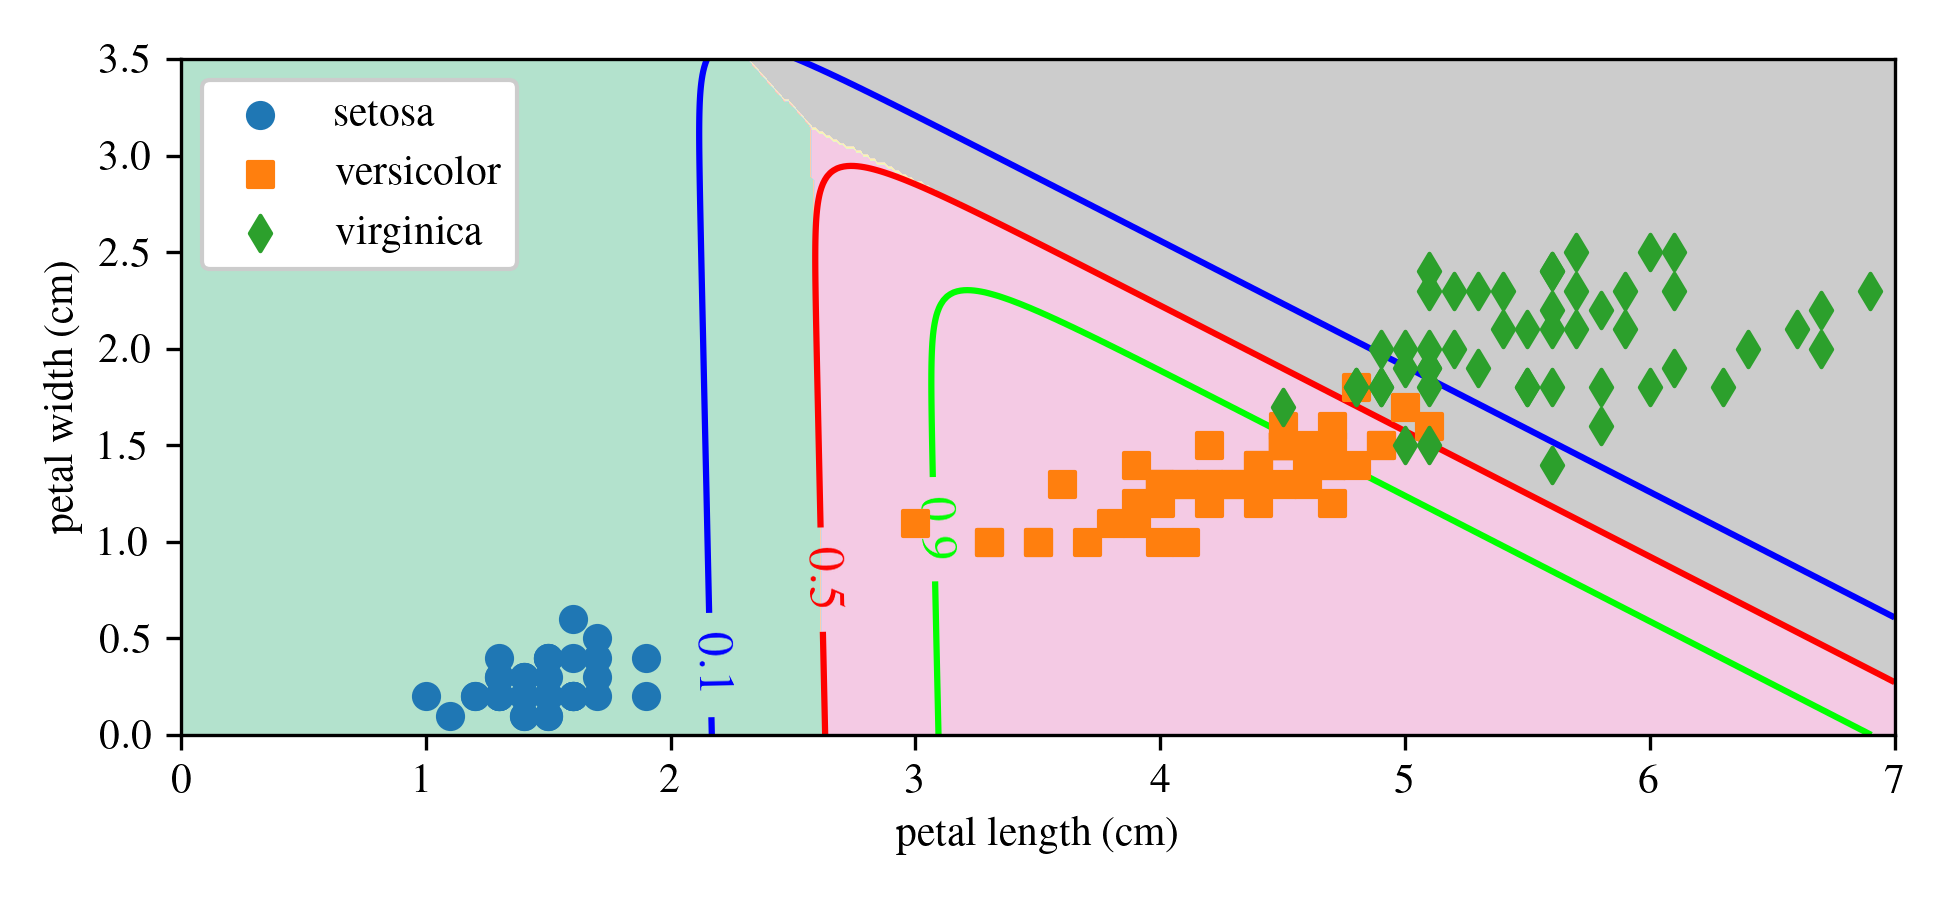
\includegraphics[width=5.5in]{../figures/Softmax_classification.png}
	\caption{Softmax classification for the three iris plant species.}
	\label{fig:Softmax_classification}
\end{figure}



\begin{example}
\textbf{Softmax Classification}

\noindent This example applies softmax regression to classify all three iris species using petal length and width. It builds a multinomial logistic regression model and visualizes the decision boundaries along with confidence contours over the 2D petal feature space.
\end{example}

\pagebreak
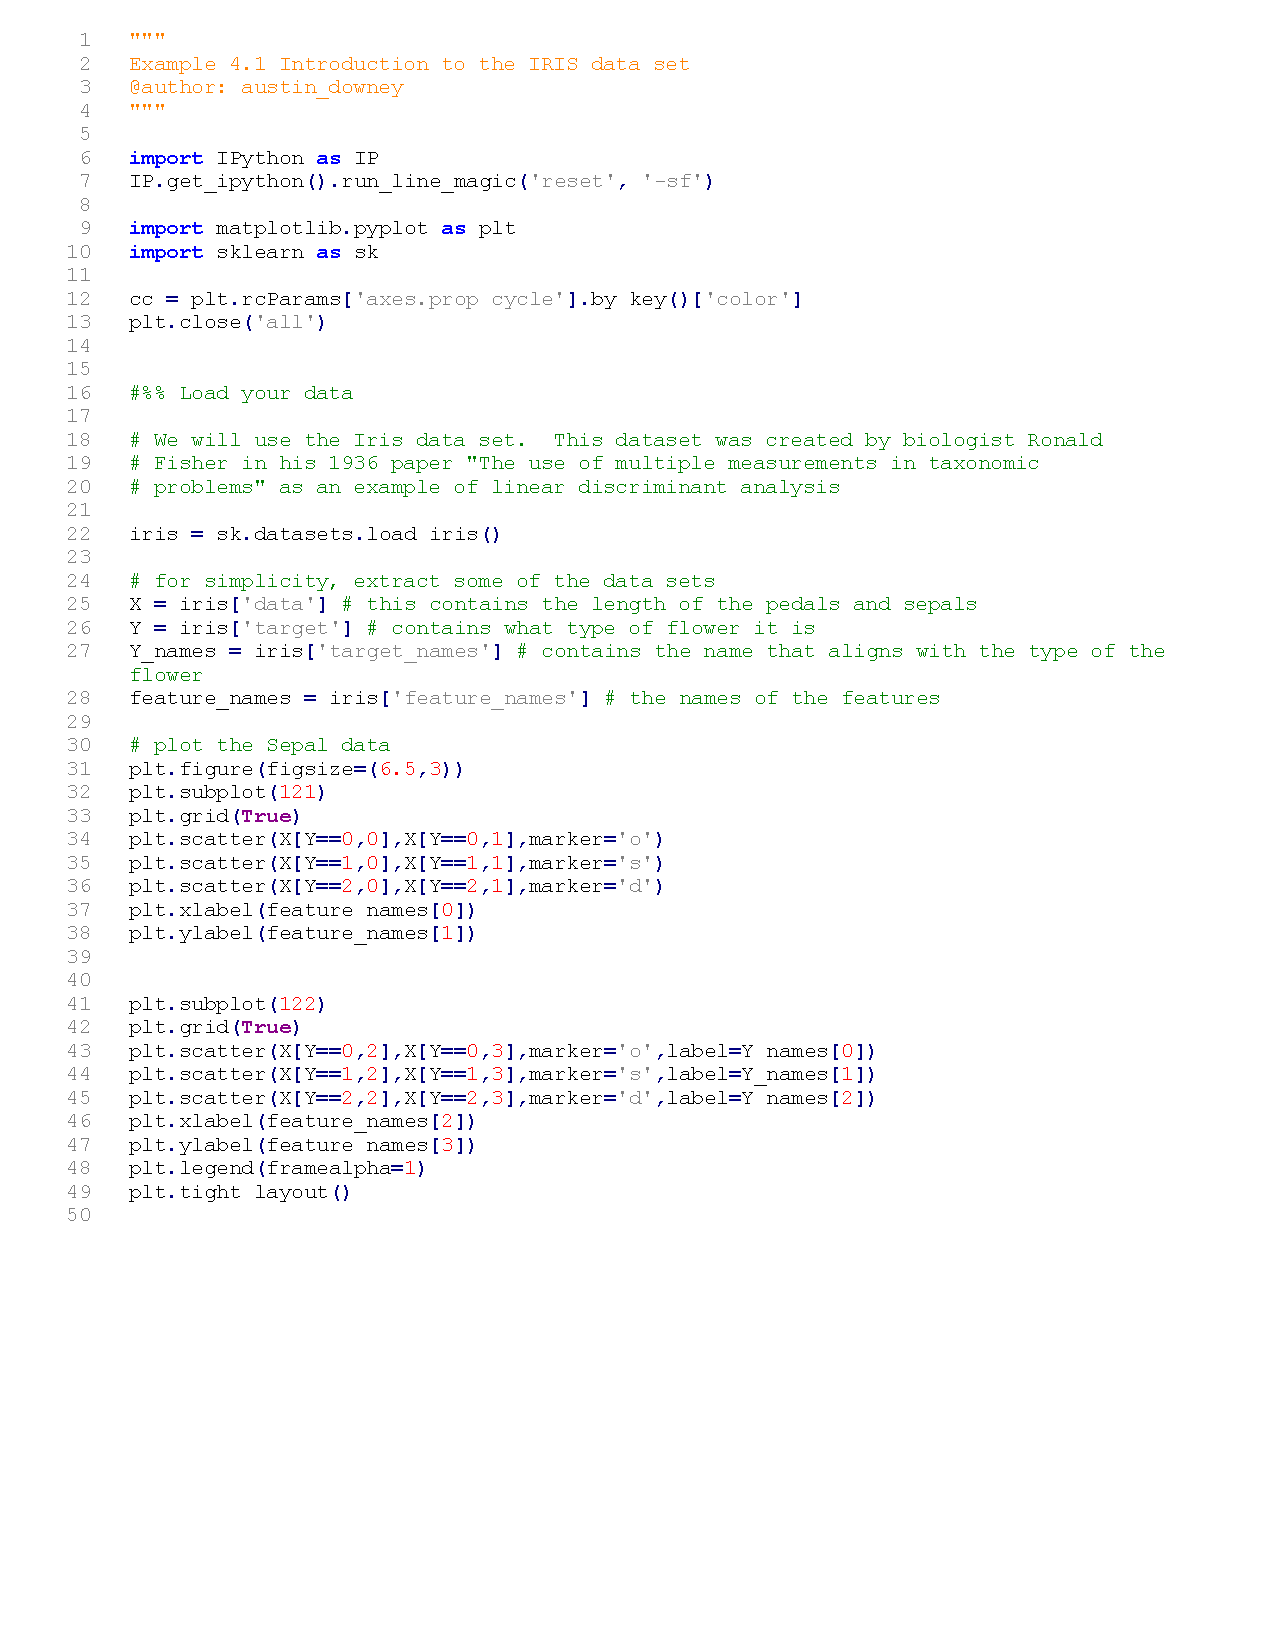
\includepdf[pages=-, width= 0.95\textwidth, pagecommand = {\subsection{Examples} \subsubsection*{Example 4.1}\vspace{0.5em}}]{../code/example_4.1_Iris_data_set.pdf}

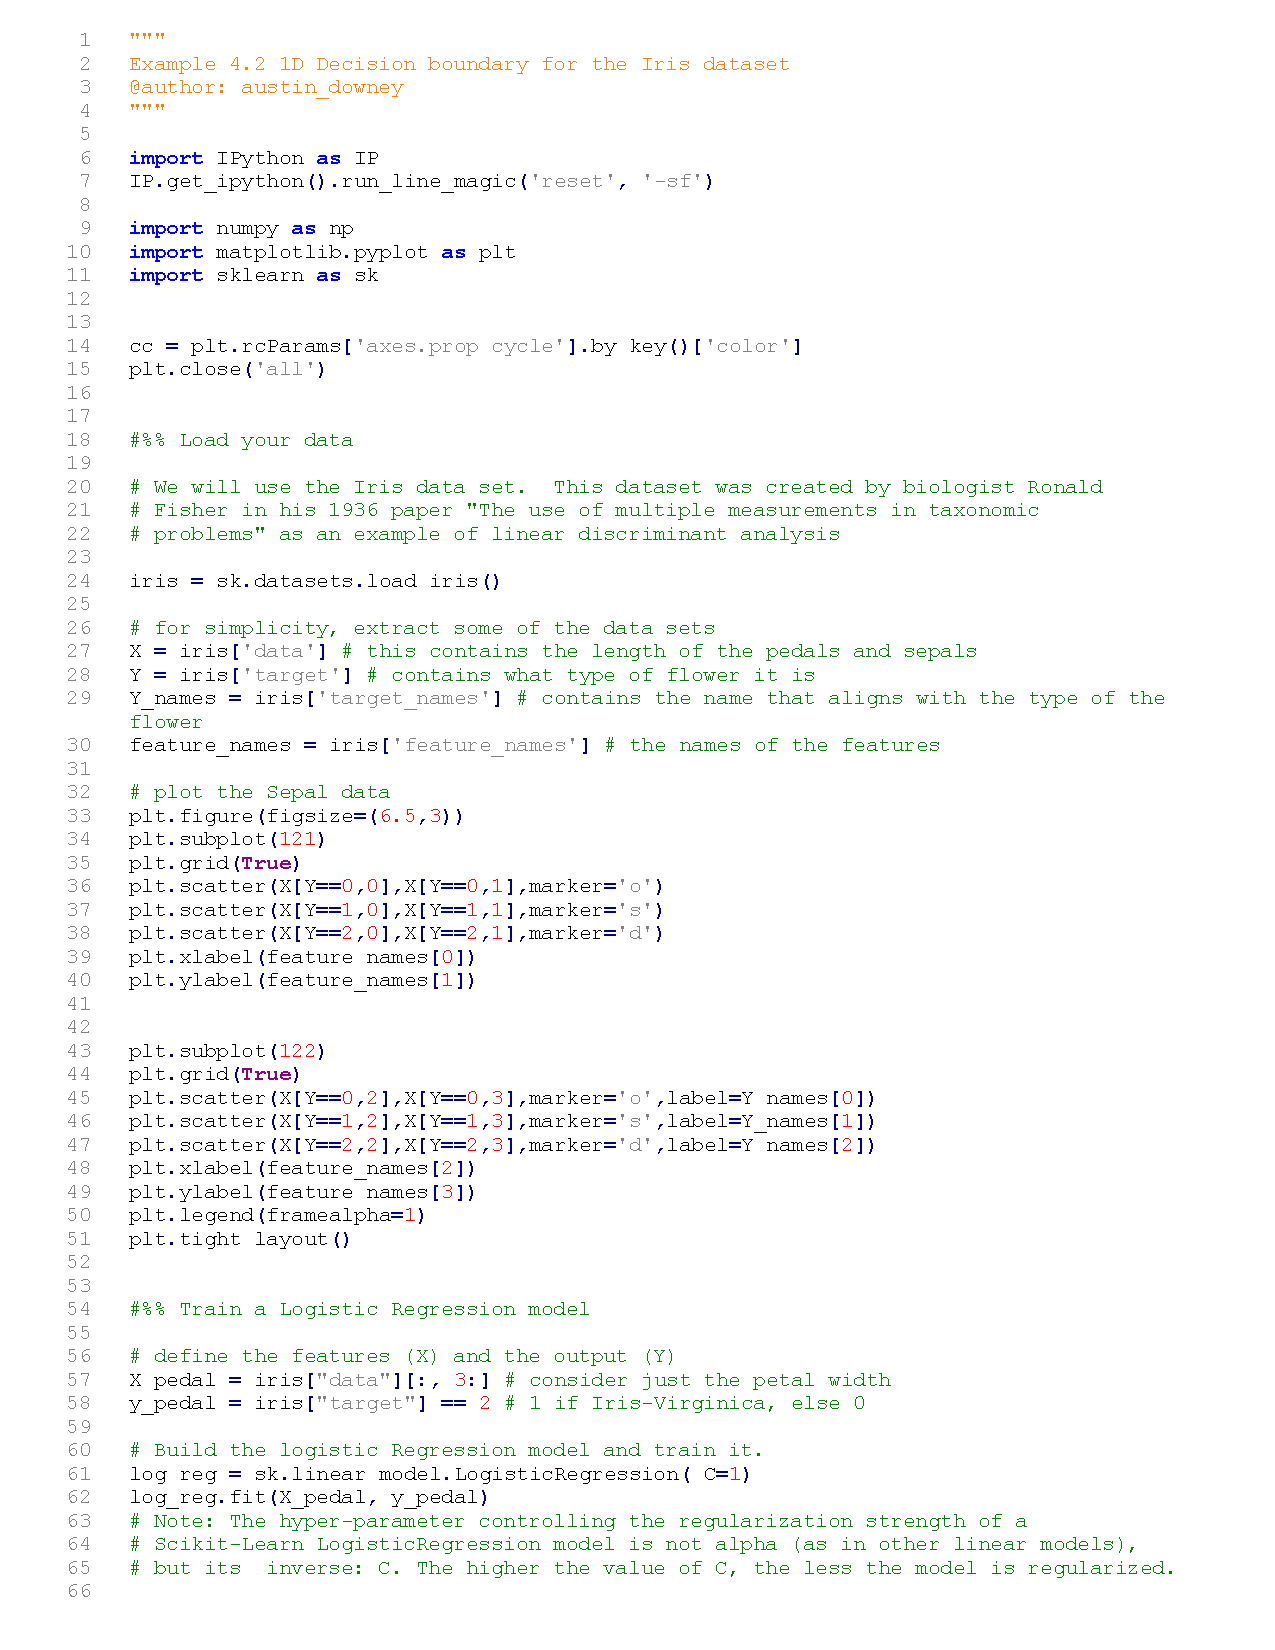
\includepdf[pages=1, width= 0.95\textwidth, pagecommand = {\subsubsection*{Example 4.2}\vspace{0.5em}}]{../code/example_4.2_Iris_1D_decision_boundary.pdf}
\includepdf[pages=2, width= 0.95\textwidth, pagecommand = {\vspace{0.5em}}]{../code/example_4.2_Iris_1D_decision_boundary.pdf}

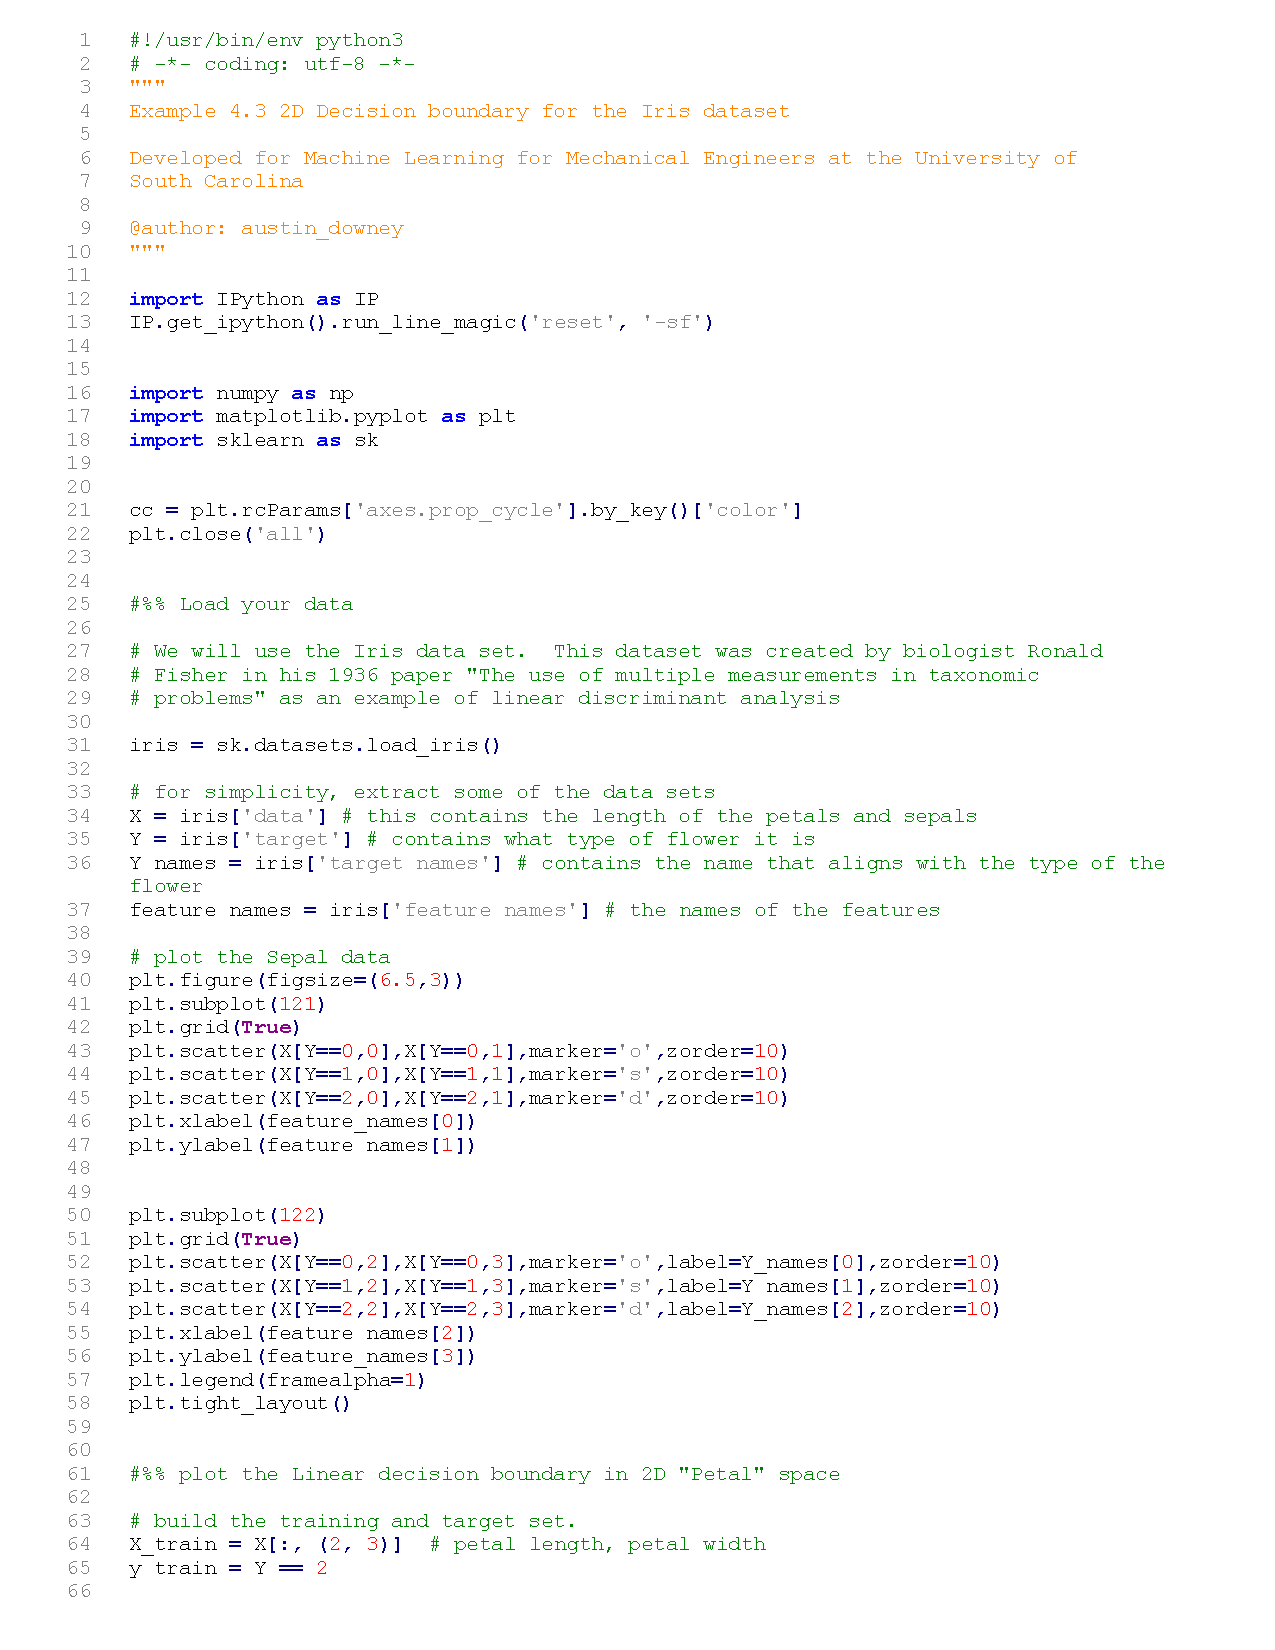
\includepdf[pages=1, width= 0.95\textwidth, pagecommand = {\subsubsection*{Example 4.3}\vspace{0.5em}}]{../code/example_4.3_Iris_2D.pdf}
\includepdf[pages=2, width= 0.95\textwidth, pagecommand = {\vspace{0.5em}}]{../code/example_4.3_Iris_2D.pdf}

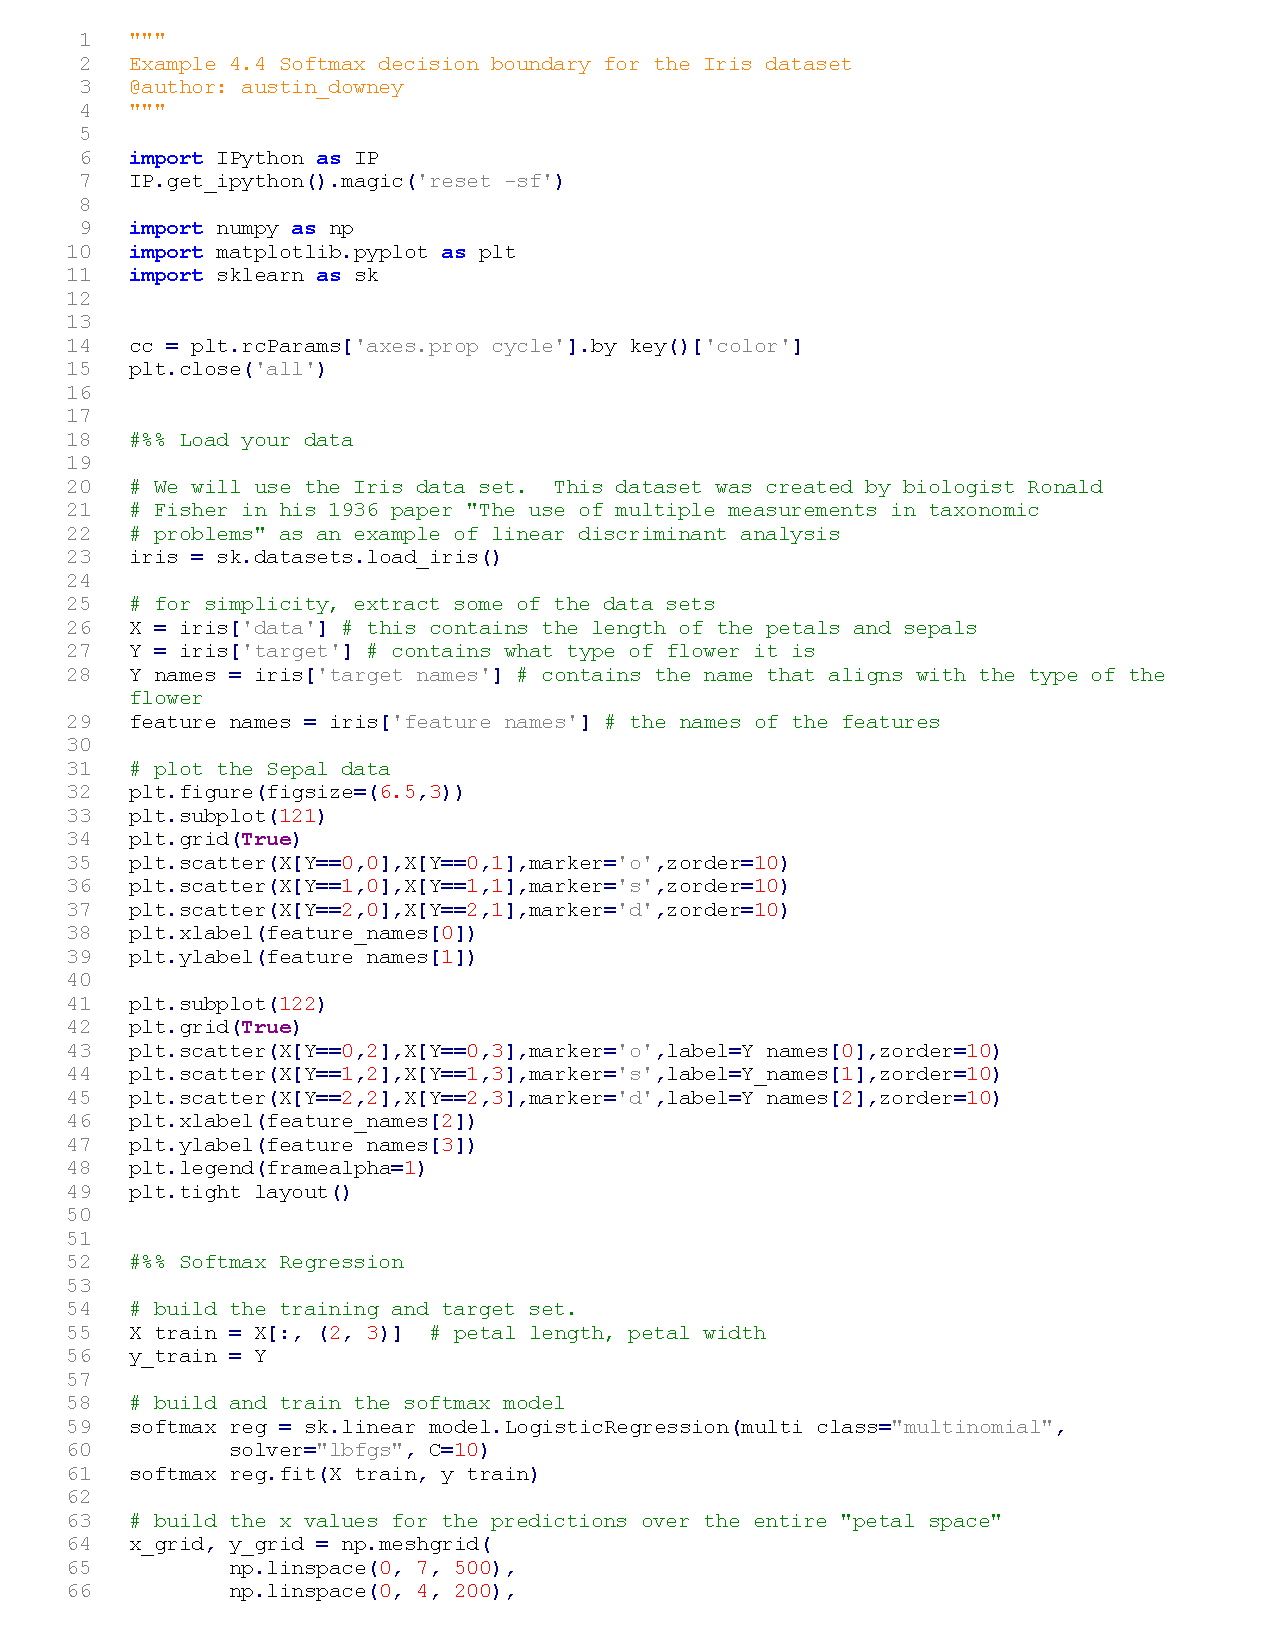
\includepdf[pages=1, width= 0.95\textwidth, pagecommand = {\subsubsection*{Example 4.4}\vspace{0.5em}}]{../code/example_4.4_softmax.pdf}
\includepdf[pages=2, width= 0.95\textwidth, pagecommand = {\vspace{0.5em}}]{../code/example_4.4_softmax.pdf}


\end{document}

